\documentclass[
 size=12pt,
 paper=smartboard, %a4paper, smartboard, screen
 mode=present, %present, handout, print
 display=slides, % slidesnotes, notes, slides
% nohandoutpagebreaks,
% pauseslide,
style=tuliplab,
% nopagebreaks,clock
% hlentries=true,
% hlsections = true,
pauseslide,
fleqn,leqno]{powerdot}

\hypersetup{pdfpagemode=FullScreen}
% \usepackage[toc,highlight,blackslide,slidesonly,sounds,HA]{HA-prosper}

\usepackage{amssymb}
\usepackage{amsmath} 
\usepackage{rotating}
\usepackage{graphicx}
\usepackage{boxedminipage}
\usepackage{media9}
\usepackage{rotate}
\usepackage{calc}
\usepackage[absolute]{textpos}
\usepackage{psfrag,overpic}
\usepackage{fouriernc}
\usepackage{pstricks,pst-node,pst-text,pst-3d,pst-grad}
\usepackage{moreverb,epsfig,color,subfigure}
\usepackage{color}
\usepackage{pstricks}
\usepackage{pstricks-add}
\usepackage{pst-text}
\usepackage{pst-node, pst-tree}
\usepackage{booktabs}
\usepackage{etex}
\usepackage{breqn}
\usepackage{multirow}
\usepackage{gitinfo2}
\usepackage{bmpsize}
\usepackage{listings}
\lstset{frameround=fttt, 
frame=trBL, 
stringstyle=\ttfamily,
backgroundcolor=\color{yellow!20},
basicstyle=\footnotesize\ttfamily}
\lstnewenvironment{code}{
\lstset{frame=single,escapeinside=`',
backgroundcolor=\color{yellow!20},
basicstyle=\footnotesize\ttfamily}
}{}

\usepackage{fouriernc}
\usepackage{hyperref}

%%%%%%%%%%%%%%%%%%%%%%%%%%%%%%%%%%%%%%%%%%%%%%%%%%%%%%%%%%%%%%%%%%%%%%%%
% title
% TODO: Customize to your Own Title, Name, Address
%
\title{FLIP(01) Mid-Term Presentation}
\author{
Jiahui Zhou
\\
Xian Shiyou University 
% \href{mailto:gangli@acm.org}{gangli@acm.org}
% \and % more authors
}
\date{\gitCommitterDate}


% Customize the setting of slides
\pdsetup{
% theslide=\arabic{slide}~/~\pageref*{lastslide},
% theslide=\arabic{slide},
rf=\href{http://www.tulip.org.au}{
Last Changed by: \textsc{\gitCommitterName}\ \gitVtagn-\gitAbbrevHash\ (\gitAuthorDate)
},
cf=\hyperlink{blankslide}{FLIP(01) Mid-Term Presentation},
trans=Fade,
list={labelsep=1em,leftmargin=*,itemsep=0pt,topsep=5pt,parsep=0pt},
% counters={theorem,lemma},
% randomdots,dmaxdots=80
}


\begin{document}

\maketitle 

\begin{slide}[toc=,bm=]{Content}
\tableofcontents[content=sections,type=1]
\end{slide}

\section{Overview}
\begin{slide}{Problem Defination}
    \begin{itemize}
        \item \textbf{Problem:}\ Google QUEST Q\&A Labeling
        \begin{itemize}
            \item Text Processing
            \item Question-answer pairs dataset
            \item Multi-task Regression
        \end{itemize}
    \end{itemize} 
    \centering{
        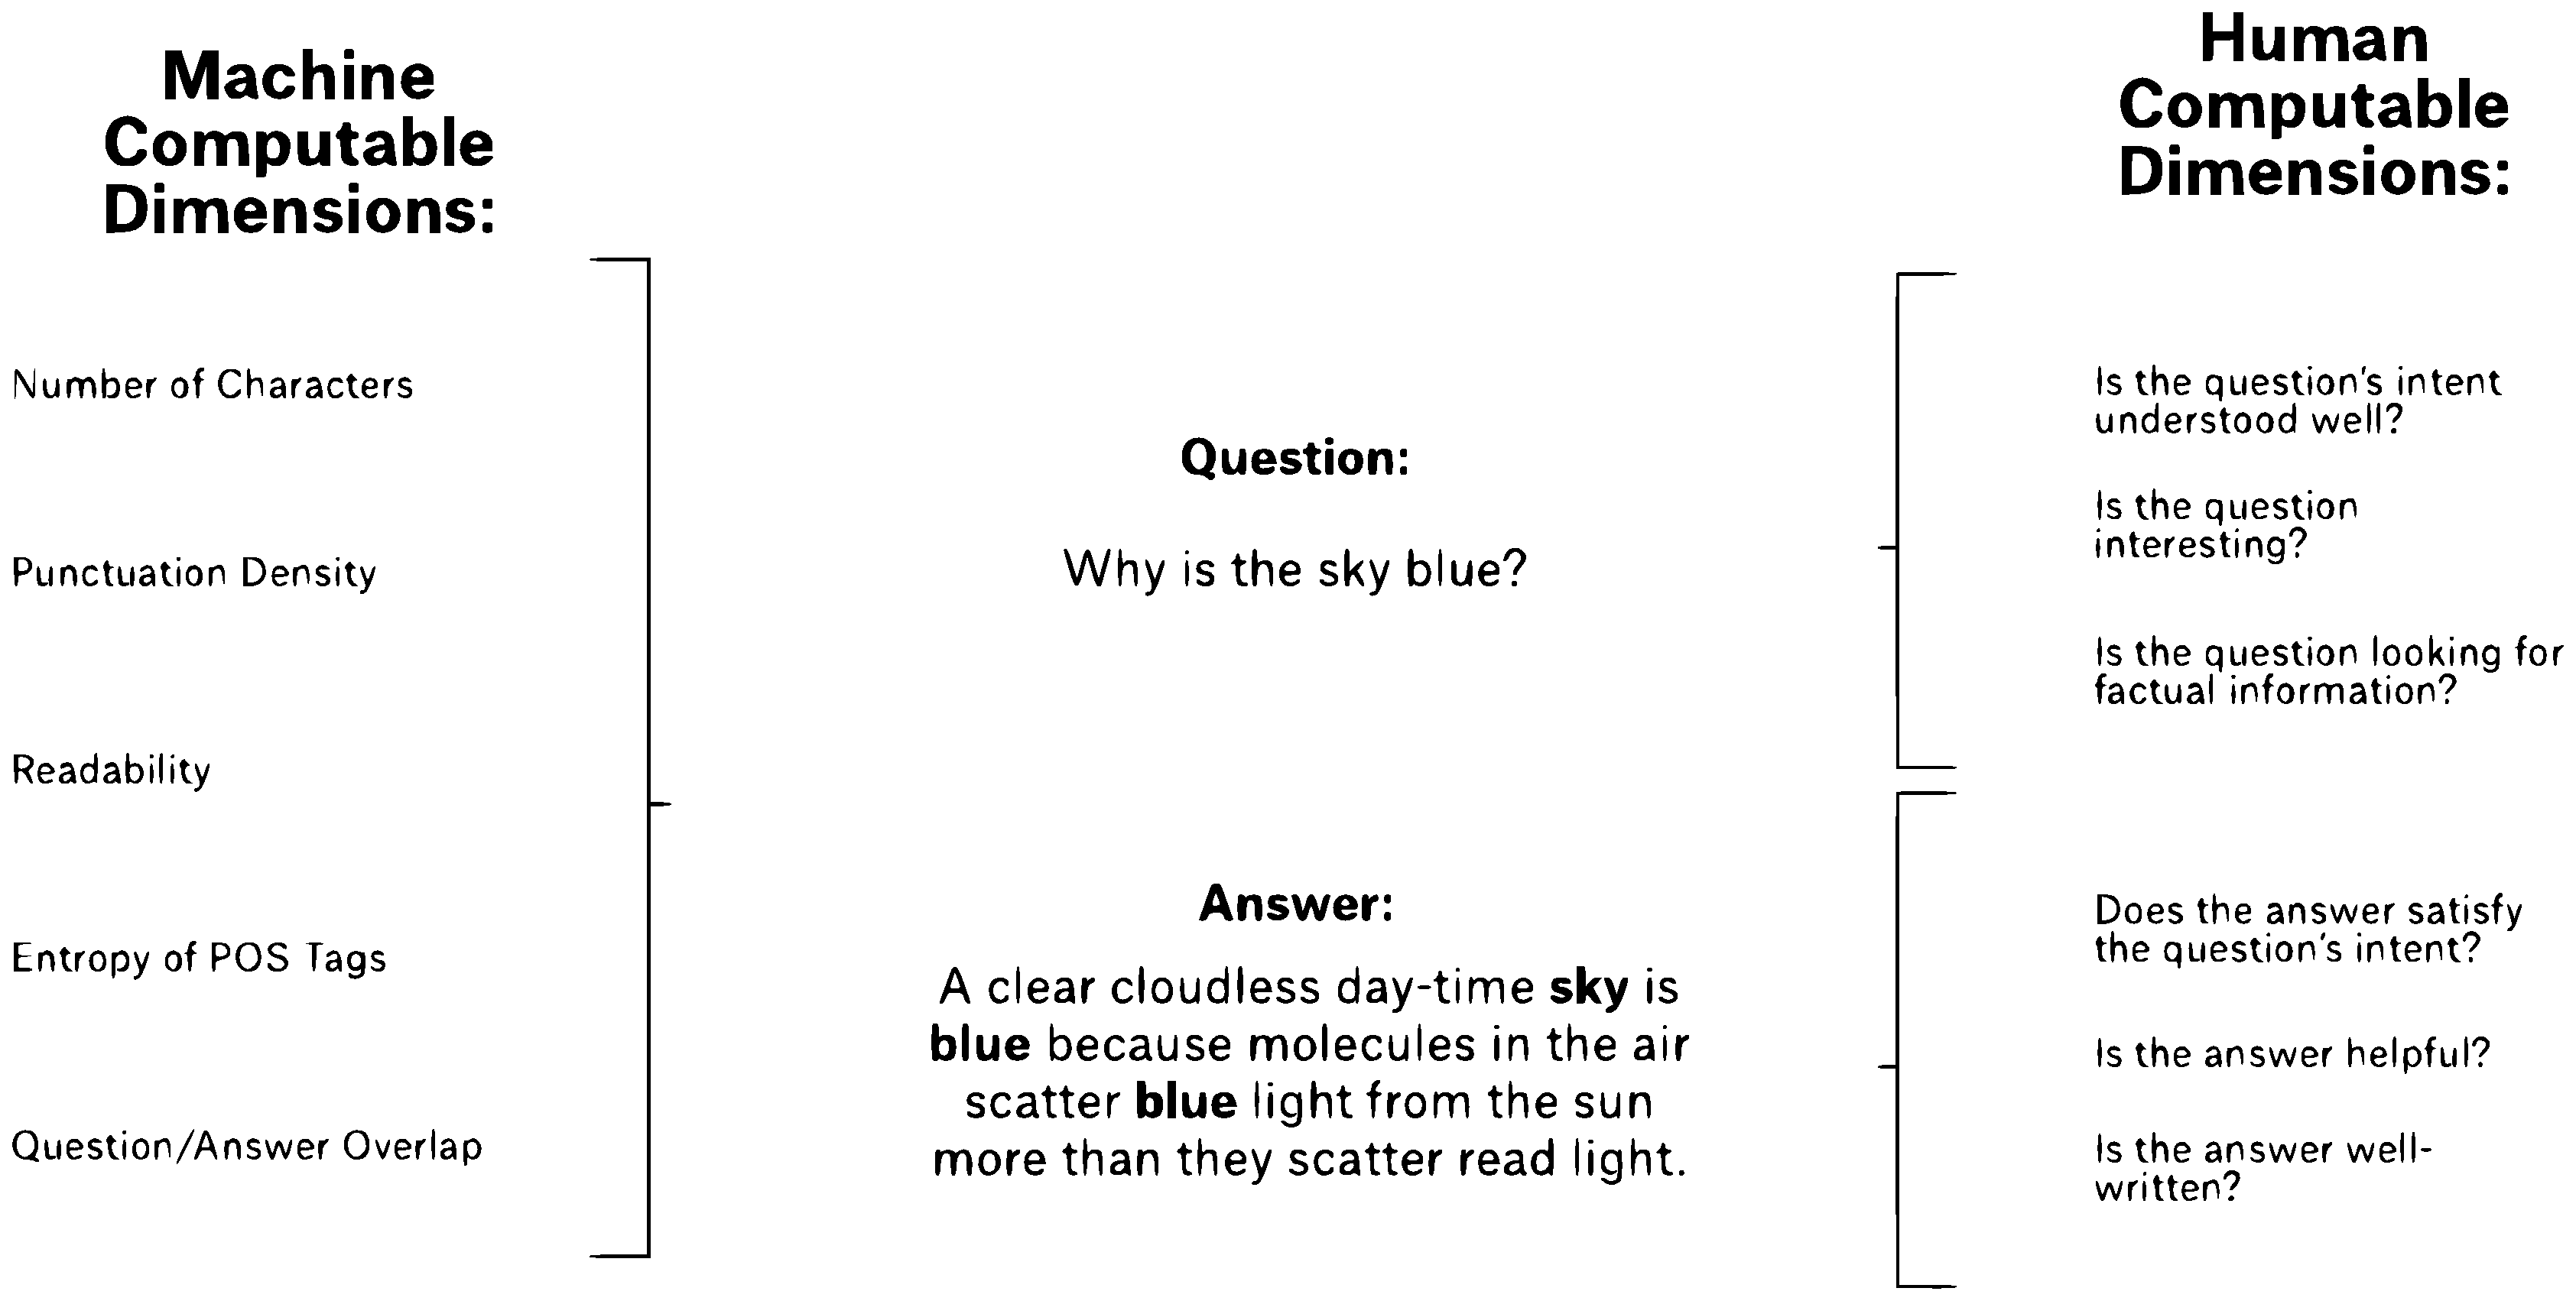
\includegraphics[height=0.5\slideheight]{figures/title.eps}  
    } 
\end{slide}
\begin{slide}{Dataset}
    \begin{itemize}
        \item Features:
        \begin{itemize}
            \item Question title\&body
            \item Answer
            \item Host
            \item Category
            \item Question user
            \item Answer user
            \item Url
        \end{itemize}
        \item Targets:
        \begin{itemize}
            \item Continuous values in the range [0,1]
            \item 21 question related target
            \item 9 answer related target
        \end{itemize}
    \end{itemize}
\end{slide}
\section{Exploring Data Analysis}
\begin{slide}{Host and Category}
    \centering{
        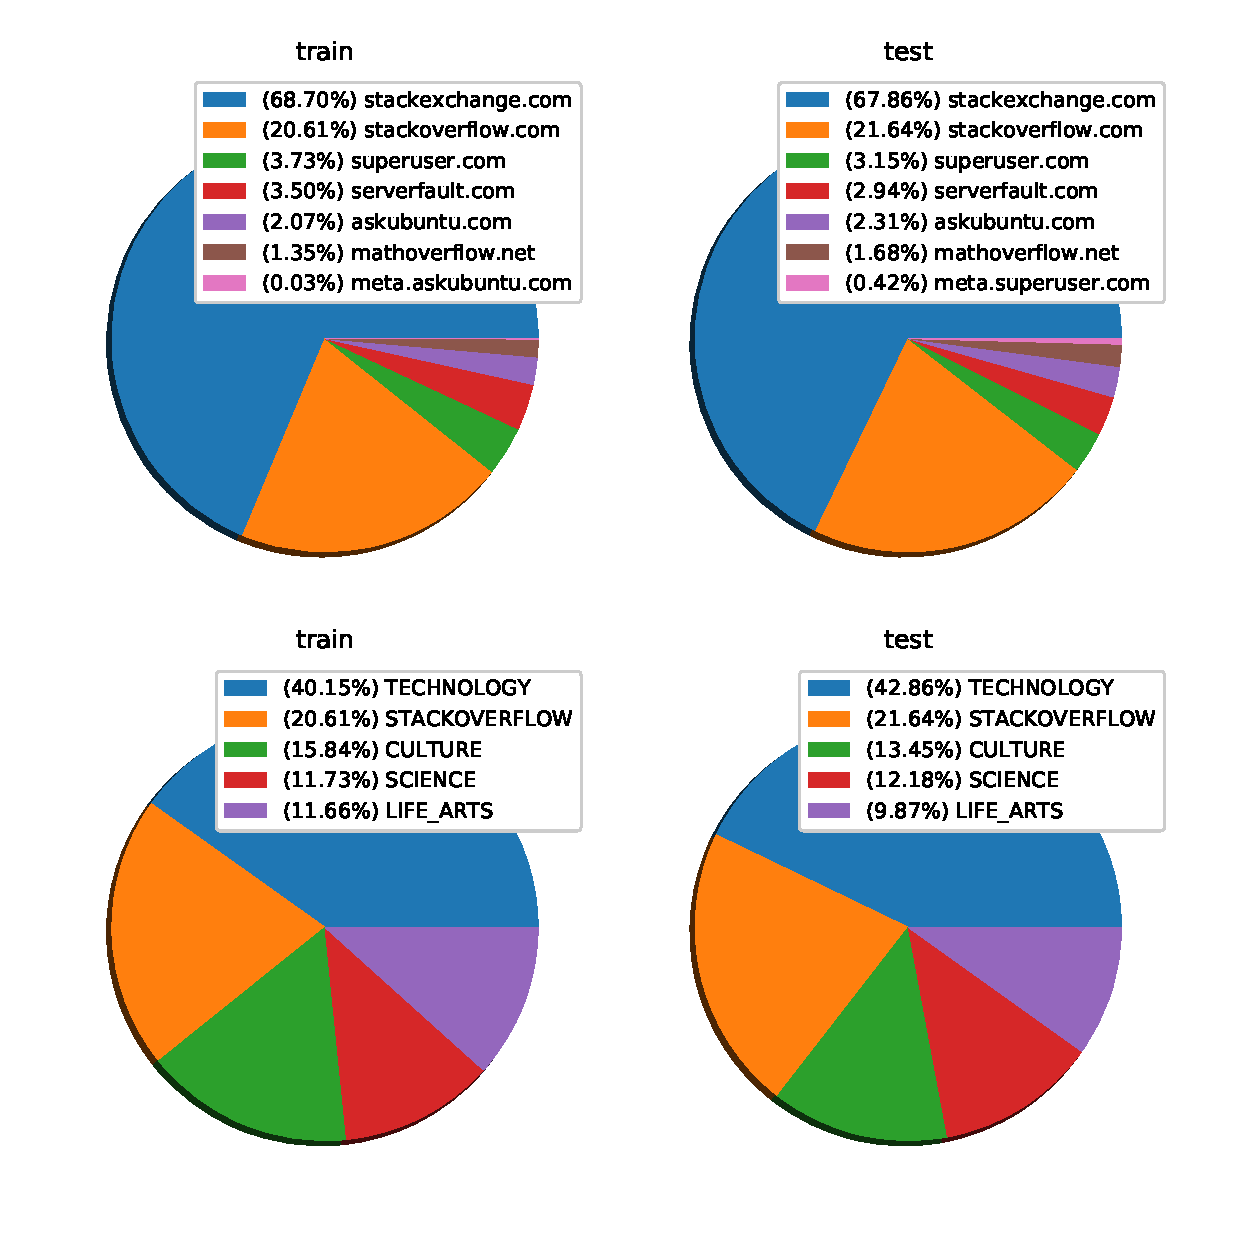
\includegraphics[height=0.6\slideheight]{figures/hosts_categories.eps}
    }
\begin{slide}{Targets}

\end{slide}
\end{slide}
\end{document}